\documentclass[ps,clariphy]{prosper} 
%\documentclass[ps]{prosper}
\usepackage[latin1]{inputenc}
\usepackage{graphicx}
\usepackage[english]{babel}
\usepackage{ulem}
\usepackage{subfig}
\usepackage{amsmath}
\usepackage{amssymb}
\usepackage{caption}
%\usepackage{caption2}
\usepackage[a4paper]{hyperref}
\usepackage{textcomp}

\graphicspath{{./graphics/}}
\hypersetup{
  pdfauthor = {Leandro Mars\'o},
  pdftitle = {},
  pdfsubject = {Flujo de Dise\~no Anal\'ogico basado en Software Libre},
  pdfkeywords = {},
  pdfcreator = {LaTeX with hyperref package},
  pdfproducer = {dvips + ps2pdf14},
  extension=pdf
}

\title{ \LARGE{Flujo de Diseno Anal\'ogico basado en Software Libre} }
\author{ Leandro Mars\'o }
\date{ Febrero 2011 }

\begin{document}
\maketitle

%%%%%%%%%%%%%%%%%%%%%%%%%%%%%%%%%%%%%%%%%%%%%%%%%%%%%%%%%%%%%%%%%%%%%%%%%%%%
% 1)  Outline
%%%%%%%%%%%%%%%%%%%%%%%%%%%%%%%%%%%%%%%%%%%%%%%%%%%%%%%%%%%%%%%%%%%%%%%%%%%%
\begin{slide}{ \textsc{{\tiny Flujo de Dise\~no Anal\'ogico basado en Software Libre}}\\ Outline}
  \vspace{-0.5cm}
  \tiny{
    \begin{itemize}
    \item Introducci\'on
      \item Flujo de dise\~no detallado
      \item Herramientas disponibles
    \item Conclusiones
      \begin{itemize}
      \item Procesos de Fabricaci\'on y Herramientas disponibles
            \item EDA and Workflow Setup %incluye como electric importa y exporta datos con otros programas (calibre drc, assura), ademas tener en cuenta quelas herramientas que se usan estan en desarrollo por lo tanto uno tiene que tener la habilidad de compilar y entender minimamente sobre el lenguaje de programacion y Makefiles. 
% Tiene que haber alguien que se encargue de hacer ejemplos de uso de cada nueva herramienta (numpy, matplot lib, etc)
	\item Propuestas
      \item Trabajo futuro %sobre flujo digital tambi\'en, pero explicitando las limitaciones que vi de alliance
      \end{itemize}
    \end{itemize}
  }
\end{slide}


%%%%%%%%%%%%%%%%%%%%%%%%%%%%%%%%%%%%%%%%%%%%%%%%%%%%%%%%%%%%%%%%%%%%%%%%%%%%
% 2) Introduction
%%%%%%%%%%%%%%%%%%%%%%%%%%%%%%%%%%%%%%%%%%%%%%%%%%%%%%%%%%%%%%%%%%%%%%%%%%%%
\begin{slide}{ \textsc{{\tiny  Flujo de Dise\~no Anal\'ogico basado en Software Libre}}\\ Introducci\'on}
  \vspace{-0.5cm}
  \tiny{
    \textbf{Introducci\'on}
    \begin{itemize}
	\item Un flujo de dise\~no est\'a compuesto por un programa espec\'ifico para cada tarea, e interfaces y formatos comunes para pasar de una etapa a la otra del dise \~no.
	\item Al mismo tiempo, seg\'un avanzan los procesos de fabricaci\'on, tambi\'en cambian las herramientas.
	\item Las herramientas fueron estudiadas por separado teniendo en cuenta la posibilidad de integraci\'on con otras, libres o no, necesario cuando se llega al punto de no encontrar herramientas libres.
	\item Teniendo encuenta estos items, y mirando los testbenches de los dise\~nadores fu\'e encarado este estudio
%    \item Europractice posee una lista de precios de herramientas no libres, para las universidades.
    \end{itemize}
  }
\end{slide}




%%%%%%%%%%%%%%%%%%%%%%%%%%%%%%%%%%%%%%%%%%%%%%%%%%%%%%%%%%%%%%%%%%%%%%%%%%%%
% 3) Introduction
%%%%%%%%%%%%%%%%%%%%%%%%%%%%%%%%%%%%%%%%%%%%%%%%%%%%%%%%%%%%%%%%%%%%%%%%%%%%
\begin{slide}{ \textsc{{\tiny Flujo de Dise\~no Anal\'ogico basado en Software Libre}}\\ Flujo de dise\~no detallado}
  \vspace{-0.5cm}
  \tiny{
\textbf{Flujo anal\'ogico:} 
    \begin{figure}[ht]
      \centering
      \scalebox{.5}{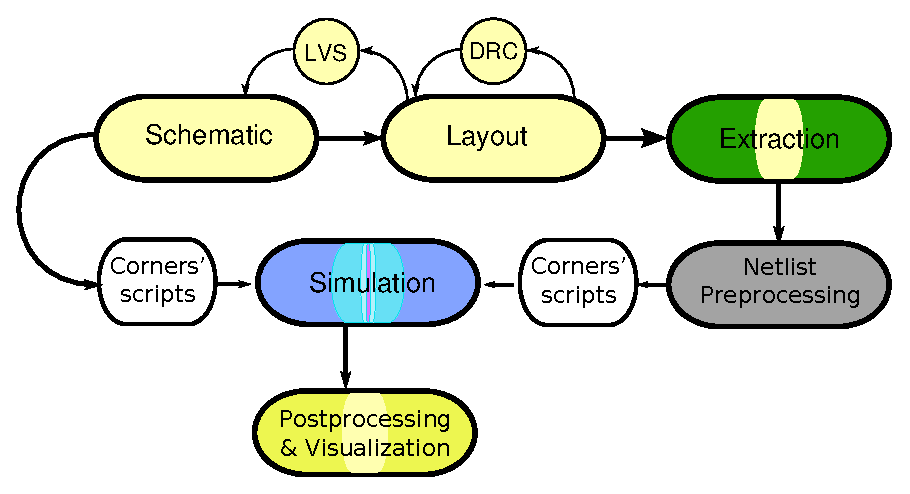
\includegraphics[angle=0]{analog-flow.eps}}
    \end{figure}
    \textbf{Tools:}
\begin{figure}[ht]
      \centering
      \scalebox{.5}{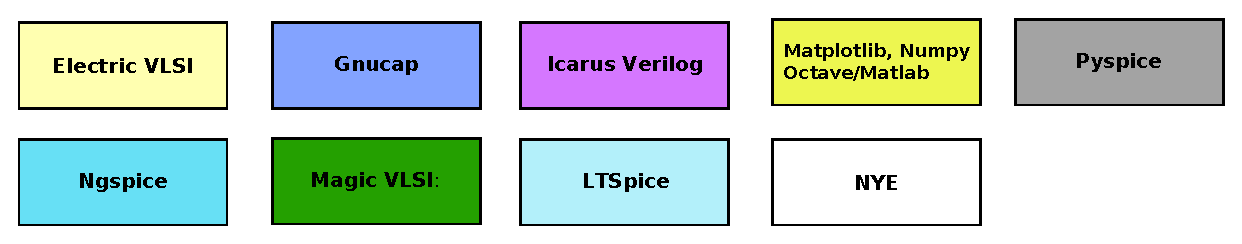
\includegraphics[angle=0]{analog-flow-tools.eps}}
    \end{figure}    
  }
\end{slide}


%%%%%%%%%%%%%%%%%%%%%%%%%%%%%%%%%%%%%%%%%%%%%%%%%%%%%%%%%%%%%%%%%%%%%%%%%%%%
% 4) Introduction
%%%%%%%%%%%%%%%%%%%%%%%%%%%%%%%%%%%%%%%%%%%%%%%%%%%%%%%%%%%%%%%%%%%%%%%%%%%%
\begin{slide}{ \textsc{{\tiny Flujo de Dise\~no Anal\'ogico basado en Software Libre}}\\ Flujo de dise\~no detallado}
  \vspace{-0.5cm}
  \tiny{
\textbf{Simulaci\'on:} 
    \begin{figure}[ht] 
%\newline 
      \centering
      \scalebox{.5}{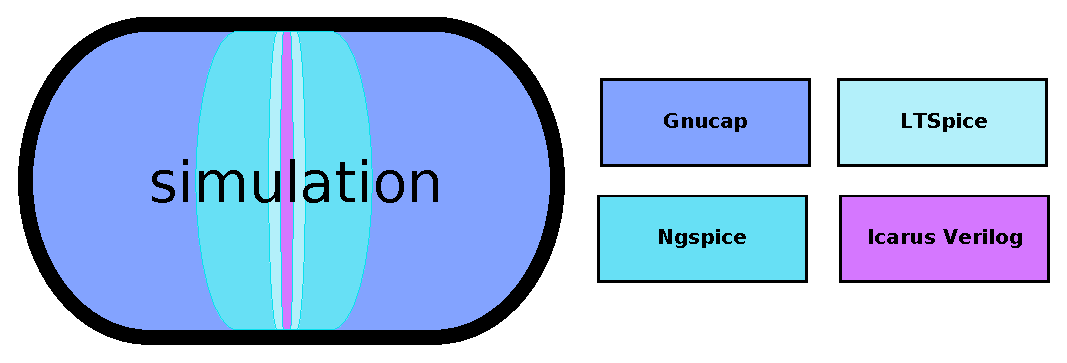
\includegraphics[angle=0]{analog-flow-simulation.eps}}
    \end{figure}
    \textbf{Herramientas necesarias:} 
\begin{itemize}
	\item Analog Simulation Engine
	\item Digital Simulation Engine
	\item Mixed Mode Simulation Engine
	\item Simulation Models: built in on simulation engine or compiled using mot-adms
    \end{itemize}
  }
\end{slide}


%%%%%%%%%%%%%%%%%%%%%%%%%%%%%%%%%%%%%%%%%%%%%%%%%%%%%%%%%%%%%%%%%%%%%%%%%%%%
% 5)  Why develop and use PCells?
%%%%%%%%%%%%%%%%%%%%%%%%%%%%%%%%%%%%%%%%%%%%%%%%%%%%%%%%%%%%%%%%%%%%%%%%%%%%
\begin{slide}{ \textsc{{\tiny Flujo de Dise\~no Anal\'ogico basado en Software Libre}}\\ Analog Simulation Engine}
  \vspace{-0.5cm}
  \tiny{
    \textbf{Gnucap:}
	\begin{itemize}
      	\item \textbf{Pros:} Fast simulator. Fully scriptable. Scales better than ngspice and LTSpice. Usefull plug-ins system to use other netlist
syntax (such as spectre, spice3f5, verilog-ams) or compile new simulation models without compiling
the whole simulator. There is a fork which implements icarus verilog cosimulation, mot-adms model compiler, among
other minor enhancements.
      	\item Due to its plug-in system, it inherits some feature improvements done on other free simulators such as ngspice. It also allows easier development of features.
      	\item Digital Verilog cosimulation is possible replacing PWL device for a verilog circuit. 
      	\item Icarus Verilog-AMS simulation will be available for cosimulation when implemented. Not there yet.
      	\item \textbf{Cons:} Lacks some simulation analisys such as noise (which is being developed now, not yet available for beta testing) or PSS.
      	\item Verilog-AMS not yet available, testbenches are more script oriented handcrafted. Coding skills needed.
	\end{itemize}
  }
\end{slide}


%%%%%%%%%%%%%%%%%%%%%%%%%%%%%%%%%%%%%%%%%%%%%%%%%%%%%%%%%%%%%%%%%%%%%%%%%%%%
% 6)  Why develop and use PCells? a9a1 z3a6q0a1a2
%%%%%%%%%%%%%%%%%%%%%%%%%%%%%%%%%%%%%%%%%%%%%%%%%%%%%%%%%%%%%%%%%%%%%%%%%%%%
\newline 
\begin{slide}{ \textsc{{\tiny Flujo de Dise\~no Anal\'ogico basado en Software Libre}}\\ Analog Simulation Engine}
\tiny{
    \textbf{Ngspice:}
	\begin{itemize}
      	\item Merges 3 different simulators: Berkeley spice3f5, Cider and Xspice which gives us a mixed-signal/mixed-level simulator.
      	\item \textbf{ Pros:} Widely used and support several analysis and compact simulation models, mot-adms model compiler can be used for verilog-ams models. Output can be
retrieved by the electric waveform viewer, or using its built-in viewer.
      	\item \textbf{Cons:} It is slower than gnucap and needs to be recompiled when a new simulation model is added.
    \end{itemize}
  %\vspace{-0.5cm}
  
    \textbf{LTSpice:}
	\begin{itemize}
      	\item The same ngspice pros and cons' applies to LTSpice. It is not free software, but its license allows it to be used for almost all industrial scenario.
    \end{itemize}
  }
\end{slide}

%%%%%%%%%%%%%%%%%%%%%%%%%%%%%%%%%%%%%%%%%%%%%%%%%%%%%%%%%%%%%%%%%%%%%%%%%%%%3544618752
% 7)  Current Pcells Developed at CASA
%%%%%%%%%%%%%%%%%%%%%%%%%%%%%%%%%%%%%%%%%%%%%%%%%%%%%%%%%%%%%%%%%%%%%%%%%%%%
\begin{slide}{ \textsc{{\tiny Flujo de Dise\~no Anal\'ogico basado en Software Libre}}\\ Schematic and Layout}
  \vspace{-0.5cm}
  \tiny{
    \textbf{Electric VLSI:}
    
      	\newline Schematic, Layout, DRC, LVS, spice netlist
\begin{itemize}
      	\item \textbf{Pros:} Actively maintained: fast bugs corrections, periodic releases with new features. 
      	\item Netlisting generator targets several simulators
      	\item Waveform viewer accepts several simulator data output
      	\item TSMC PDK avaiable for 180nm, 90nm and 45nm and even can export cells to SKILL 
	\item Can read DRC error output from Cadence and Menotor tools
	 
      	\item \textbf{Cons:} Schematic lacks finger/multiplier params, Layout is done in a different way, but easy to learn
\end{itemize}
  }
\end{slide}

% 8)  Current Pcells developed at CASA
\begin{slide}{ \textsc{{\tiny Flujo de Dise\~no Anal\'ogico basado en Software Libre}}\\ Schematic and Layout}
  \vspace{-0.5cm}
  \tiny{
    \textbf{Magic VLSI:}
    \newline We use only \textbf{parasitic extraction} and netlist generation feature of this layout tool
\begin{itemize}
      	\item \textbf{Pros:} More accurate than Electric, widely used for old processes (0.25um and above)
\item \textbf{Cons:} Need to write another techfile for this tool
\item Not acceptable for nanometer processes.Schematic, Layout, DRC, LVS, spice netlist
\end{itemize}
  }
\end{slide}


%%%%%%%%%%%%%%%%%%%%%%%%%%%%%%%%%%%%%%%%%%%%%%%%%%%%%%%%%%%%%%%%%%%%%%%%%%%%%%%%%%%%%%%%%%%%%%%%%%%%%
% 8
%%%%%%%%%%%%%%%%%%%%%%%%%%%%%%%%%%%%%%%%%%%%%%%%%%%%%%%%%%%%%%%%%%%%%%%%%%%%%%%%%%%%%%%%%%%%%%%%%%

\begin{slide}{ \textsc{{\tiny Flujo de Dise\~no Anal\'ogico basado en Software Libre }}\\Postprocesamiento y visualizaci\'on }
  \vspace{-0.5cm}
\tiny{
  \textbf{Cadence calculator replacement:}
\newline \textbf{Numpy} library can be used as a tool to postprocess simulation results (ascii data in gnucap and spice raw format in ngspice) It is a matlab replacement also. 
\newline \textbf{Matplolib} is a library that can be used to view the simulation results. Electric waveform viewer can be used also (not for gnucap results)

\begin{itemize}
      	\item Pros: Very flexible tools, known as a easy replacement for matlab 
      	\item Cons: This methodology can be slower for designers that are used to Cadence tools. CAD engineer or the designer should prepare a set of common task before start designing.
\end{itemize}
}
\end{slide}

%%%%%%%%%%%%%%%%%%%%%%%%%%%%%%%%%%%%%%%%%%%%%%%%%%%%%%%%%%%%%%%%%%%%%%%%%%%%%%%%%%%%%%%%%%%%%%%%%%%%%
%  9 
%%%%%%%%%%%%%%%%%%%%%%%%%%%%%%%%%%%%%%%%%%%%%%%%%%%%%%%%%%%%%%%%%%%%%%%%%%%%%%%%%%%%%%%%%%%%%%%%%%

\begin{slide}{ \textsc{{\tiny Flujo de Dise\~no Anal\'ogico basado en Software Libre}}\\ Netlist preprocessing}
  \vspace{-0.5cm}
  \tiny{
 \textbf{pyspice:} This tool can do some reduction on parallel transistor and capacitors to help low down number of nodes on post extraction netlist, to reduce simulation time. 

	}
\end{slide}


%%%%%%%%%%%%%%%%%%%%%%%%%%%%%%%%%%%%%%%%%%%%%%%%%%%%%%%%%%%%%%%%%%%%%%%%%%%%
% 11) Current Pcells developed at CASA
%%%%%%%%%%%%%%%%%%%%%%%%%%%%%%%%%%%%%%%%%%%%%%%%%%%%%%%%%%%%%%%%%%%%%%%%%%%%
\begin{slide}{ \textsc{{\tiny Flujo de Dise\~no Anal\'ogico basado en Software Libre}}\\ Conclusions}
  \vspace{-0.5cm}
  \tiny{
\textbf{Summary\': Technology process versus available tools} 
    \begin{figure}[ht]
      \centering

      \scalebox{0.6}{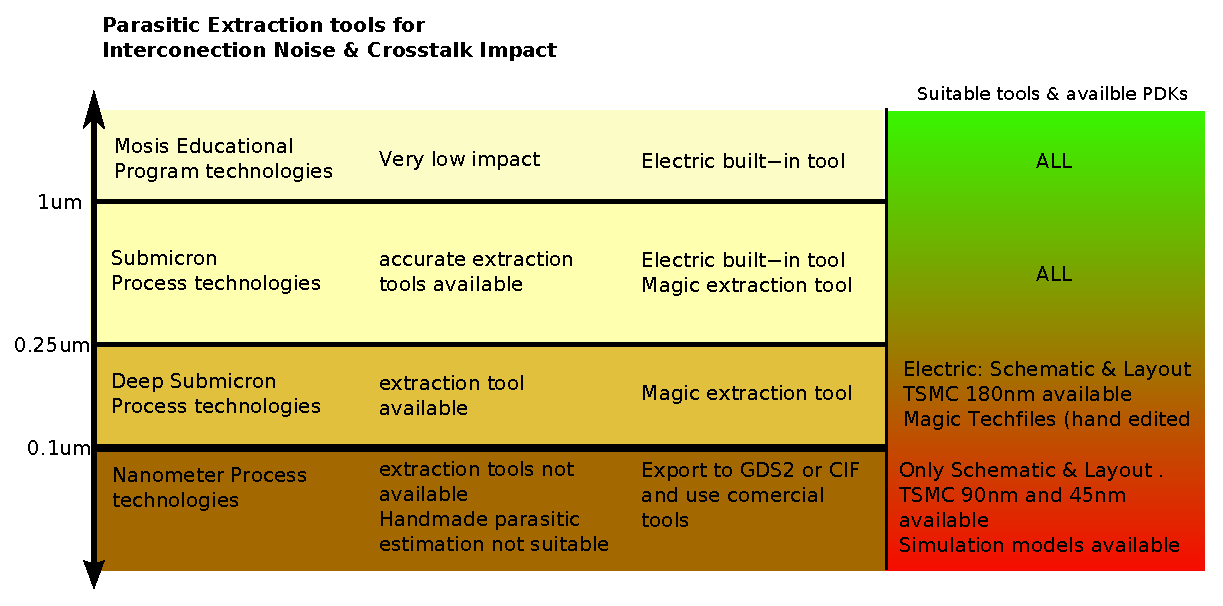
\includegraphics[angle=0]{parasitic-extraction.eps}}
    \end{figure}

  	

  }
  
\end{slide}


%%%%%%%%%%%%%%%%%%%%%%%%%%%%%%%%%%%%%%%%%%%%%%%%%%%%%%%%%%%%%%%%%%%%%%%%%%%%%%%%%%%%
% 12 Current Pcell developed at CASA
%%%%%%%%%%%%%%%%%%%%%%%%%%%%%%%%%%%%%%%%%%%%%%%%%%%%%%%%%%%%%%%%%%%%%%%%%%%%%%%%%%%%
\begin{slide}{ \textsc{{\tiny Flujo de Dise\~no Anal\'ogico basado en Software Libre}}\\ Conclusions }
  \vspace{-0.5cm}
\tiny{ EDA and workflow setup
  \begin{figure}[ht]
      \centering
      \scalebox{0.4}{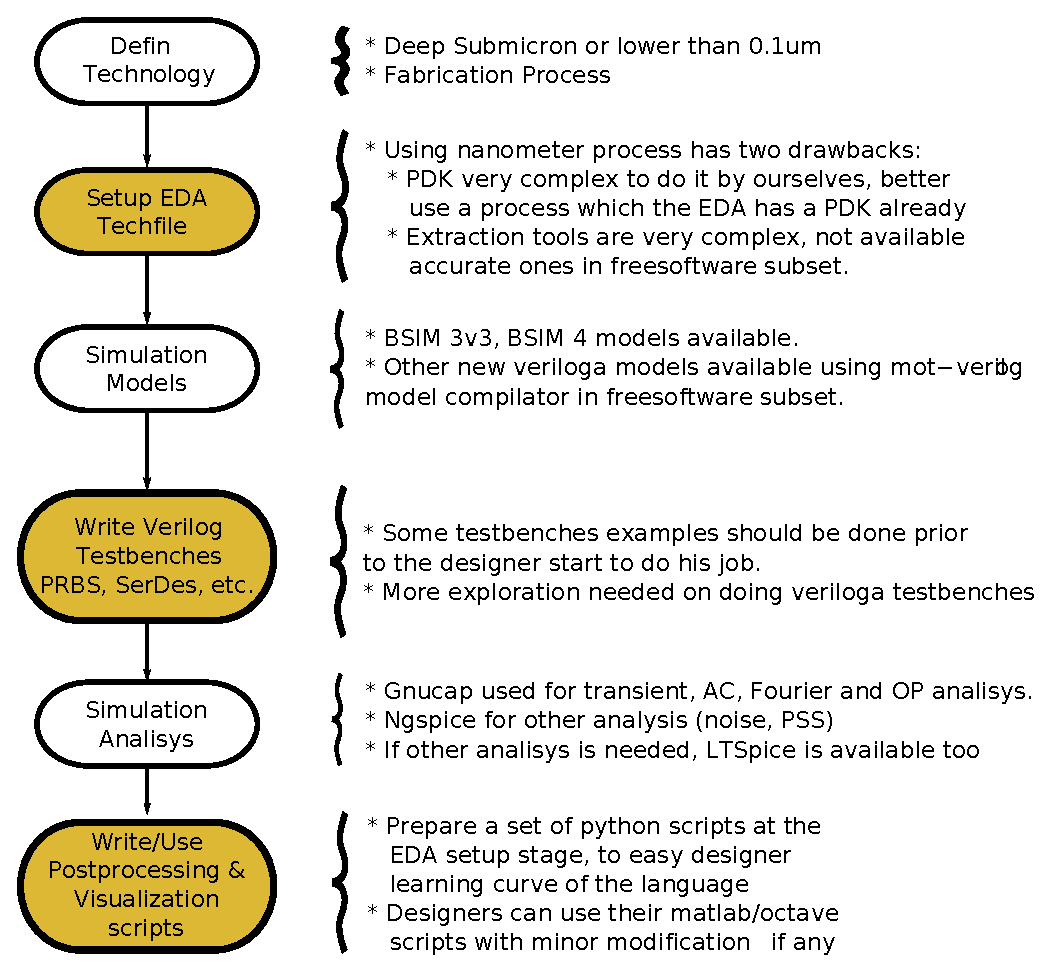
\includegraphics[angle=0]{EDA-setup.eps}}
    \end{figure}
}
\end{slide}








%%%%%%%%%%%%%%%%%%%%%%%%%%%%%%%%%%%%%%%%%%%%%%%%%%%%%%%%%%%%%%%%%%%%%%%%%%%%%%%%%%%%
% 13 Current Pcell developed at CASA
%%%%%%%%%%%%%%%%%%%%%%%%%%%%%%%%%%%%%%%%%%%%%%%%%%%%%%%%%%%%%%%%%%%%%%%%%%%%%%%%%%%%



\begin{slide}{ \textsc{{\tiny Flujo de Dise\~no Anal\'ogico basado en Software Libre}}\\ Conclusions}
  \vspace{-0.5cm}
  \tiny{
\begin{itemize}
\item Before start choosing a tool, process technology must be defined.
\item Tools can be replaced one by one, not necesary to forge an entirely custom workflow.
\item Tasks more likely to being replaced Cadence workflow is schematic and layout design, depending on the technology process.
\item Most of these tools are actively developed, so it is recommended (if not compulsory) compiling and coding skills.
% Tiene que haber alguien que se encargue de hacer ejemplos de uso de cada nueva herramienta (numpy, matplot lib, etc)
%Tiene que haber alguien que se encargue de hacer ejemplos de uso de cada nueva herramienta (numpy, matplot lib, etc)
\item To help ease the change, well documented examples for every task should be available (expecially for numpy, matplotlib and handcrafted testbenches scripts)
\item Previous survey on asitic turns to be very usefull now.

 \end{itemize}
  }
\end{slide}


%%%%%%%%%%%%%%%%%%%%%%%%%%%%%%%%%%%%%%%%%%%%%%%%%%%%%%%%%%%%%%%%%%%%%%%%%%%%%%%%%%%%
% 14 Trabajo futuro
%%%%%%%%%%%%%%%%%%%%%%%%%%%%%%%%%%%%%%%%%%%%%%%%%%%%%%%%%%%%%%%%%%%%%%%%%%%%%%%%%%%%



\begin{slide}{ \textsc{{\tiny Flujo de Dise\~no Anal\'ogico basado en Software Libre}}\\ Conclusions}
  \vspace{-0.5cm}
  \tiny{
\textbf{Future work}
\begin{itemize}
\item Test simulator with large nets to be sure that we don't hit a tool limit when doing production everday work. We should be able to use extracted netlist from QRC Cadence of a real block designed in CASA.
\item Try to export data to allow visibility of CASA blocks for INC database.

 \end{itemize}
  }
\end{slide}




\end{document}
